\documentclass[a4paper,14pt]{extreport}

\newcommand{\globalEncoding}{utf8}		% кодировка	
\newcommand{\globalStylesDir}{"E:/Documents/Git/graduateWorkStyle"}	% месторасположение стилей
\newcommand{\globalSourceDir}{src}	% месторасположение кодов
\newcommand{\globalPictureDir}{pic}	% месторасположение изображений

% подключаем набор стилей
\usepackage{\globalStylesDir/graduateWorkMain}



\begin{document}
	% Tитульная страница
	\title{Разработка ПО для автоматизации конфигурирования сетевого оборудования CISCO}
	\subtitle{Отчет по преддипломной практике}
	\teachers{2}{Трофимов С.П.}
	\students{1}{Черетаев И.В.}
	\specialty{Информатика и вычислительная техника}
	\group{РИ-420207}
	\city{Екатеринбург}		
	\maketitle
	\setcounter{page}{2} % начать нумерацию страниц с №2
	
	% Оглавление
	\tableofcontents
	
	\chapter*{Введение}
	\addcontentsline{toc}{chapter}{ВВЕДЕНИЕ}
	
	Во второй половине прошлого века в связи с «рождением» первых
	вычислительных сетей произошла очередная научно-техническая революция. Появилась возможность начать использование рассредоточенной
	обработки данных, обширно использовать для автоматизации различных
	видов деятельности новые технологии. В наши дни даже маленький ребенок имеет представление о компьютерных сетях, и, в то же время,
	наладка сетевого оборудования является довольно кропотливым делом,
	которое не терпит небрежного отношения.
	
	В наше время происходит активное применение сетевых решений во многих сферах деятельности. В условиях производства, на различных предприятиях,
	в офисах компаний, различных фирмах и учреждениях отдельно стоящий, не подключенный к сети компьютер является большой редкостью. Можно смело заявлять, что через какое-то время
	большая часть компьютеров будет включено в те или иные сети. Если же
	подобной сети в учреждении нет или она плохо развита, нет сомнений,
	что ей придется развиваться.
	
	Основным моментом в данном вопросе является технический прогресс, постоянно обеспечивающий нас новыми возможностями, но накладывающим на технических специалистов высокие требования, в частности – необходимость повышенной адаптивности. Несмотря на это,
	для специалистов наладка сетевого оборудования являет собой одно из
	основных направлений, где качество безоговорочно удерживает пальму
	первенства по важности.
	
	Одним из представителей компаний-производителей сетевого оборудования является Cisco Systems. Cisco Systems — компания-производитель
	сетевого оборудования, основанная в 1984. Сначала компания производила маршрутизаторы, но затем значительно расширила ассортимент своей продукции. В настоящее время она производит коммутаторы, маршрутизаторы,
	IP-телефоны, программное обеспечение для своего оборудования.
	
	Огромное сообщество сетевых администраторов, IT-специалистов, студентов не всегда хочет привлекать квалифицированных специалистов
	Cisco для того, чтобы быстро запустить какой-либо проект на оборудовании Cisco. Они обычно нуждается в простом, работающем решении,
	позволяющее им не посвящать остаток жизни изучению всех тонкостей сетевых технологий, маршрутизации, информационной безопасности, беспроводной связи и т.д.
	
	Соответственно, необходимо решение, которое быстро и легко поможет настроить оборудование Cisco и решить данные проблемы.
	
	\chapter{Техническое задание}
	
	\section{Общие положения}
	
	\subsection{Наименование программы}
	
	Программное обеспечение для автоматизации конфигурирования сетевого оборудования Cisco. Условное обозначение – АКСО\cite{gost-19.201-78}.
	
	\subsection{Краткая характеристика области применения}
	
	АКСО предназначено для частичной или полной автоматизации процесса изменения исходного текста с целью получения отличного от первоначального стиля изложения.
	
	\subsection{Основание для проведения разработки}
	Перечень документов, на основании которых ведется разработка надстройки:
	
	\begin{enumerate}
		\item Приказ ректора УрФУ № \_\_\_\_\_\_ от "\_\_\_"\_\_\_\_\_\_\_\_\_\_ \_\_\_\_\_г.
	\end{enumerate}
		
	Порядок оформления и предъявления результатов проектирования устанавливается согласно документам:
	
	\begin{enumerate}
		\item  Методические указания по выполнению выпускной квалификационной работы бакалавра техники и технологий по направлению "Информатика и вычислительная техника" / сост. А.Б.Николаев. – Москва: МАДИ, 2010. – 17 с.
		\item Методические указания к выполнению выпускных бакалаврских работ по направлению 552800 «Информатика и вычислительная техника» по специальности 230101 65 «Вычислительные машины, комплексы, системы, сети»/Под общей ред.В.А.Бархоткина. - Москва:МИЭТ, 2006. - 15с.
		\item Соколов С.С. Рекомендации по оформлению курсовых, выпускных и дипломных проектов (работ). Электронные методические указания - Екатеринбург: Изд. УрФУ, 2010. - 38 с.
	\end{enumerate}
	
	
	\section{Назначение разработки}
	
	\subsection{Функциональное назначение}
	Функциональным предназначением АКСО является предоставлению пользователю удобных инструментов для облегчения конфигурирования сетевого оборудования от компании Cisco Systems, таких как маршрутизаторы и/или коммутаторы.
	
	\subsection{Эксплуатационное назначение}
	
	АКСО предназначено для автоматизации процесса конфигурирования сетевого оборудования с целью получения исходного текста конфигурации либо автоматического применения внесенных с помощью АКСО изменений на сетевом оборудовании. Пользователями АКСО могут являться системные администраторы, сетевые инженеры, студенты.
	
	\section{Требования к программному средству}
	
	\subsection{Требования к функциональным характеристикам}
	
	\begin{enumerate}
		\item Разработать структуру классов, хранящую информацию о сетевых устройствах.
		
		\item Ввести основные модели маршрутизаторов и коммутаторов.
		
		\item Разработать редактор, позволяющий добавлять новые модели (в том числе, на основе уже существующих моделей), изменять и удалять существующие. Редактор должен обеспечивать возможность поиска в списке имеющихся моделей. Так же при помощи данного редактора должны производиться операции визуального изменения конфигурации для выбранного модели сетевого оборудования.
		
		\item Разработать систему для экпорта/импорта выбранной конфигурации в виде XML-файла, содержащего все необходимые сведения.
		
		\item Разработать систему для сохранения выбранной конфигурации в виде текстового файла, содержащего команды конфигурирования
		
		\item Разработать справочную подсистему. Справка должна содержать краткую информацию о системе и ее возможностях, описание действий пользователя и получаемых результатов при работе с программным обеспечением.
		
		\item Реализовать перечисленные выше функции в рамках приложения для настольного компьютера с графическим интерфейсом.
	\end{enumerate}
	
	\subsection{Требования к надежности функционирования и безопасности}
	
	Надёжность системы должна обеспечивать работоспособность в течение всего срока эксплуатации при бесперебойном питании ЭВМ. Наработка на отказ при эксплуатации программного средства должна составлять не менее 8 часов. Программное обеспечение не должно содержать явных логических ошибок и функционировать без сбоев.
	
	В течение срока эксплуатации необходимо выполнение требований «ГОСТ 51188-98. Защита информации. Испытания программных средств на наличие компьютерных вирусов».
	
	\subsection{Требования к составу и параметрам технических средств}
	В состав технических средств должна входить ЭВМ, включающая в себя:
	
	\begin{itemize}
		\item процессор с тактовой частотой не менее  1 ГГц;
		\item ОЗУ не менее 512 МБ;
		\item экран с разрешением не менее 1024x768 точек;
		\item клавиатура;
		\item манипулятор «мышь».
	\end{itemize}	
	
	\subsection{Требования к информационной и программной совместимости}
	
	АКСО должна иметь возможность функционировать под управлением различных операционных систем (Windows, Linux и т.д.).
	
	\subsection{Требования к исходным кодам и языкам программирования}
	
	В ходе прохождения преддипломной практики необходимо выбрать на каком языке программирования будет написан исходный код программного средства, а также интегрированную среду разработки.
	
	\subsection{Специальные требования}
	
\begin{itemize}
	\item 	Программа должна обеспечивать взаимодействие с пользователем (оператором) посредством графического пользовательского интерфейса.
\end{itemize}
	
	\section{Требования к программной докуменации}
	\subsection{Предварительный состав программной документации}
	\label{subsection:documentation}
	Предварительный состав программной документации должен включать в себя\cite{gost-19.105-78,gost-19.106-78}:
\begin{enumerate}
	\item техническое задание;
	\item текст программы;
	\item описание программы;
	\item программу и методики испытаний;
	\item пояснительную записку\cite{methodVKR,methodVKR2,methodVKRUrFU};
	\item описание применения;
	\item руководство пользователя.
\end{enumerate}
	
	\section{Стадии и этапы разработки}
	
	\subsection{Стадии разработки}
	
	Разработка должна быть произведена в три стадии\cite{gost-19.102-77}:
	\begin{enumerate}
		\item Разработка технического задания;
		\item Рабочее проектирование;
		\item Внедрение;
	\end{enumerate}
	
	\subsection{Этапы разработки}
	На стадии рабочего проектирования должны быть выполнены перечисленные ниже этапы работ:
	\begin{enumerate}
		\item разработка АКСО; 
		\item разработка программной документации; 
		\item испытания АКСО.
	\end{enumerate}
	
	На стадии внедрения должен быть выполнен этап разработки - подготовка АКСО.
	
	\subsection{Содержание работ по этапам}
	
	На этапе разработки АКСО должна быть выполнена работа по программированию (кодированию) и отладке программного обеспечения (АКСО).
	
	На этапе разработки программной документации должна быть выполнена разработка программных документов в соответствии с требованием п. \ref{subsection:documentation} настоящего технического задания.
	
	На этапе испытаний АКСО должны быть выполнены перечисленные ниже виды работ:
	
	\begin{enumerate}
		\item проверка выполнения заданных функций АКСО;
		\item выявления и устранения недостатков в АКСО и программной документации; 
		\item корректировка АКСО и программной документации по результатам тестирований\cite{gost-28195-89}.
	\end{enumerate}
	
	На этапе подготовки АКСО должна быть выполнена работа по подготовке программного средства и программной документации для эксплуатации.
	
	\section{Порядок защиты и контроля}
	
	Защита осуществляется перед Государственной аттестационной комиссией (ГАК), утвержденной приказом ректора.
	
%	\section{Источники разработки}
%	\begin{enumerate}
%		\item ГОСТ 19.201-78. Техническое задание, требования к содержанию и оформлению. 
%		\item ГОСТ 19.102-77 ЕСПД. Стадии разработки. 
%		\item ГОСТ 19.104-78 ЕСПД. Основные надписи. 
%		\item ГОСТ 19.105-78 ЕСПД. Общие требования к программным документам. 
%		\item ГОСТ 19.106-78 ЕСПД. Требования к программным документам, выполненным печатным способом. 
%		\item ГОСТ 28195-89. Оценка качества программных средств. Общие положения.
%		\item ГОСТ 19.781-90. Обеспечение систем обработки информации программное. Термины и определения
%		\item  Методические указания по выполнению выпускной квалификационной работы бакалавра техники и технологий по направлению "Информатика и вычислительная техника" / сост. А.Б.Николаев. – Москва: МАДИ, 2010. – 17 с.
%		\item Методические указания к выполнению выпускных бакалаврских работ по направлению 552800 «Информатика и вычислительная техника» по специальности 230101 65 «Вычислительные машины, комплексы, системы, сети»/Под общей ред.В.А.Бархоткина. - Москва:МИЭТ, 2006. - 15с.
%		\item Соколов С.С. Рекомендации по оформлению курсовых, выпускных и дипломных проектов (работ). Электронные методические указания - Екатеринбург: Изд. УрФУ, 2010. - 38 с.
%		\item ISO/IEC 12207:1995 (ГОСТ Р) Информационные технологии. Процессы жизненного цикла программного обеспечения.
%		\item ISO/IEC 9126:1991 (ГОСТ Р) Информационные технологии. Оценка программного продукта. Характеристики качества и порядок их применения.
%	\end{enumerate}
	
	\chapter{Выбор инструментальной системы}
	
	Приложения для настольных компьютеров в значительной степени зависят от платформы, на которой они работают. Приложение, скомпилированное для ОС Linux, не может работать в другой операционной системе без использования эмуляторов по причине различий в системных вызовах и библиотеках в этих операционных системах. Необходимо было найти возможность разработки платформонезависимых приложений.
	 
	Одним из методов является разработка версий библиотек для всех необходимых платформ, не изменяя код приложения, а просто перекомпилируя его для каждой платформы. Этот подход облегчал жизнь разработчикам до того момента, как компания Sun Microsystems представила революционную концепцию виртуальных машин, подарив миру платформонезависимый язык программирования Java. Приложения Java исполняются при помощи виртуальной машины Java (Java Virtual Machine). Код, написанный однажды, может быть развернут на любой платформе, для которой доступна виртуальная машина Java.
	 
	Но за все приходится платить. В случае с языком Java приходится расплачиваться производительностью. Производительность приложений на Java не настолько высока, как у приложений на C/C++, скомпилированных в машинный код. Другим недостатком является большое потребление памяти этими приложениями. Без сомнения, язык Java занимает лидирующие позиции, но на сегодняшний день существуют приложения, обрабатывающие большие объемы данных (например, в области биотехнологии) с особо жесткими требованиями к производительности. И снова мы сталкиваемся с необходимостью разработки приложений, компилируемых в машинный код. Разработка приложений на языке C занимает много времени, в то время как C++ является лучшим решением. Имеется ряд фреймворков, предназначенных для использования при разработке приложений на C++. Фреймворк Qt является одним из них. 
	
	Qt позволяет запускать написанное с его помощью ПО в большинстве современных операционных систем путём простой компиляции программы для каждой ОС без изменения исходного кода. Включает в себя все основные классы, которые могут потребоваться при разработке прикладного программного обеспечения, начиная от элементов графического интерфейса и заканчивая классами для работы с сетью, базами данных и XML. Qt является полностью объектно-ориентированным, легко расширяемым и поддерживающим технику компонентного программирования.
	
	Отличительная особенность Qt от других библиотек — использование Meta Object Compiler (MOC) — предварительной системы обработки исходного кода. MOC позволяет во много раз увеличить мощь библиотек, вводя такие понятия, как слоты и сигналы. Кроме того, это позволяет сделать код более лаконичным. Утилита MOC ищет в заголовочных файлах на C++ описания классов, содержащие макрос Q\_OBJECT, и создаёт дополнительный исходный файл на C++, содержащий метаобъектный код.
	
	Qt позволяет создавать собственные плагины и размещать их непосредственно в панели визуального редактора. Также существует возможность расширения привычной функциональности виджетов, связанной с размещением их на экране, отображением, перерисовкой при изменении размеров окна.
	
	Qt комплектуется визуальной средой разработки графического интерфейса «Qt Designer», позволяющей создавать диалоги и формы в режиме WYSIWYG. В поставке Qt есть «Qt Linguist» — графическая утилита, позволяющая упростить локализацию и перевод программы на многие языки; и «Qt Assistant» — справочная система Qt, упрощающая работу с документацией по библиотеке, а также позволяющая создавать кросс-платформенную справку для разрабатываемого на основе Qt ПО. Начиная с версии 4.5.0 в комплект Qt включена среда разработки «Qt Creator», которая включает в себя редактор кода, справку, графические средства «Qt Designer» и возможность отладки приложений. «Qt Creator» может использовать GCC или Microsoft VC++ в качестве компилятора и GDB в качестве отладчика. Для Windows версий библиотека комплектуется компилятором, заголовочными и объектными файлами MinGW.

	\chapter{Обзор существующих решений}
	
	Существует достаточно большое количество симуляторов и эмуляторов для оборудования Cisco Systems.
	В ходе  показать все существующие инструменты, которые решают эту задачу.
	
	Вначале немного терминологии.
	
	Симуляторы — имитируют некий набор команд, он вшит и стоит только выйти за рамки, сразу получим сообщение об ошибке. Классический пример — Cisco Packet Tracer.
	
	Эмуляторы же напротив — позволяют проигрывать (выполняя байт трансляцию) образы (прошивки) реальных устройств, зачастую без видимых ограничений. В качестве примера — GNS3/Dynamips.
	
	\section{Cisco Packet Tracer}
	
	Packet Tracer — симулятор сети передачи данных, выпускаемый фирмой Cisco Systems. Позволяет делать работоспособные модели сети, настраивать (командами Cisco IOS) маршрутизаторы и коммутаторы, взаимодействовать между несколькими пользователями (через облако). В симуляторе реализованы серии маршрутизаторов Cisco 800, 1800, 1900, 2600, 2800, 2900 и коммутаторов Cisco Catalyst 2950, 2960, 3560, а так же межсетевой экран ASA 5505. Беспроводные устройства представлены маршрутизатором Linksys WRT300N, точками доступа и сотовыми вышками. Кроме того есть серверы DHCP, HTTP, TFTP, FTP, DNS, AAA, SYSLOG, NTP и EMAIL, рабочие станции, различные модули к компьютерам и маршрутизаторам, IP-фоны, смартфоны, хабы, а так же облако, эмулирующее WAN. Объединять сетевые устройства можно с помощью различных типов кабелей, таких как прямые и обратные патч-корды, оптические и коаксиальные кабели, последовательные кабели и телефонные пары.
	
	Этот симулятор доступен как под Windows, так и для Linux, бесплатно для учащихся Сетевой Академии Cisco.
	
	Его плюсы — дружественность и логичность интерфейса. Кроме этого в нем удобно проверять работу разных сетевых сервисов, вроде DHCP/DNS/ HTTP/SMTP/POP3 и NTP.
	И одна из самых интересных фич — это возможность перейти в режим simulation и увидеть перемещения пакетов с замедлением времени.
	
	Однако, стоит заметить, что реализованная функциональность устройств ограничена и не предоставляет всех возможностей реального оборудования. Практически всё, что выходит за рамки CCNA, на нем собрать не получится. К примеру, EEM отсутствует напрочь.
	
	\begin{figure}[h!]
	\centering
	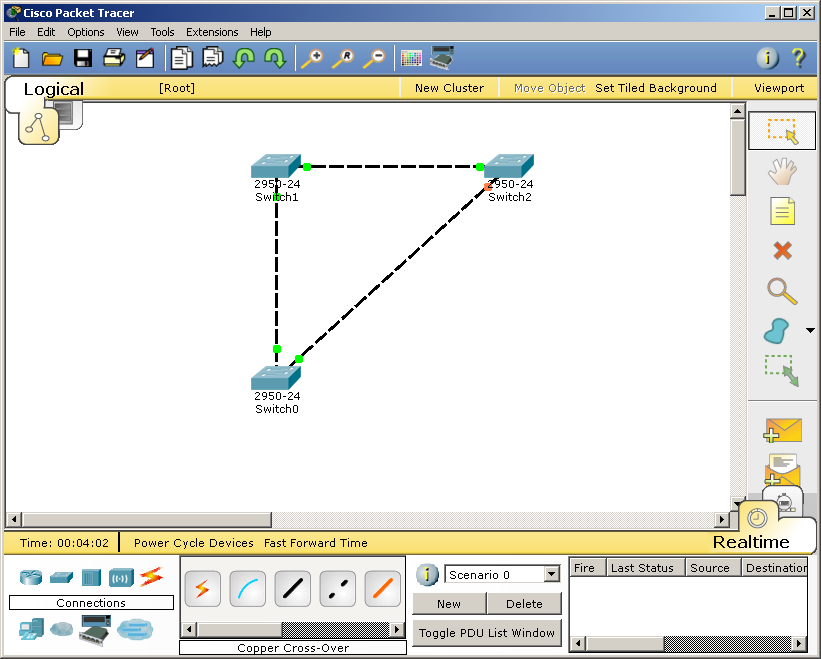
\includegraphics[width=0.9\linewidth]{pic/packet_tracer}
	\caption{Cisco Packet Tracer}
	\label{fig:packet_tracer}
	\end{figure}
		
	\section{GNS3}
	
	
	Следующий — GNS3, который представляет собой графический интерфейс (на Qt) для эмулятора dynamips.
	
	
	
	Свободный проект, доступен под Linux, Windows и Mac OS X.
	
	\begin{figure}[h!]
	\centering
	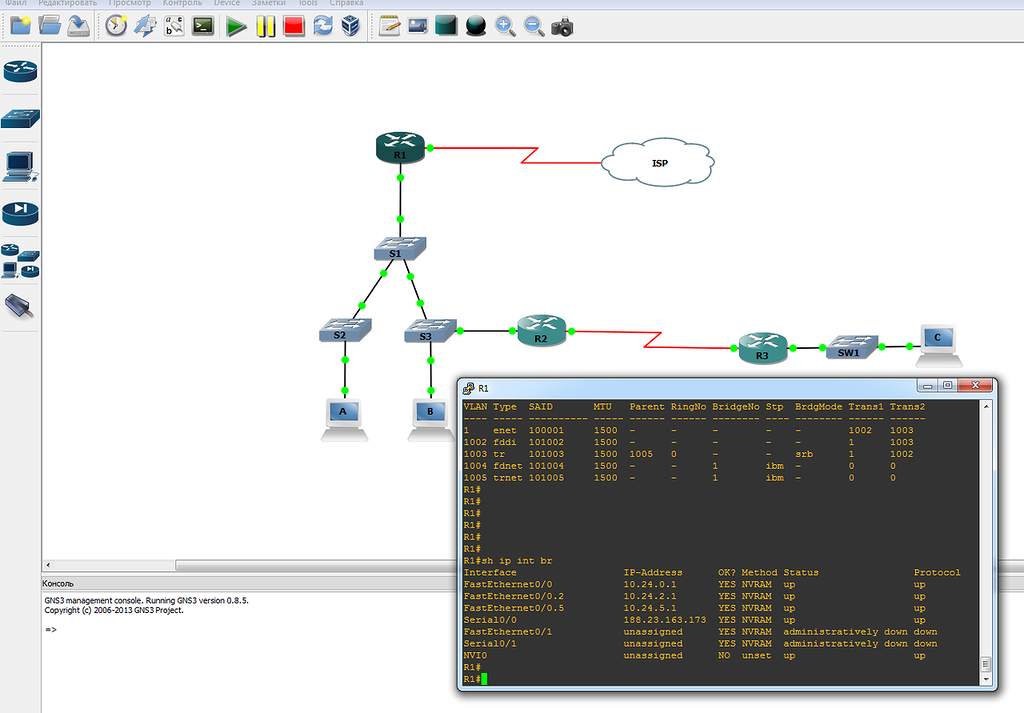
\includegraphics[width=0.9\linewidth]{pic/gns3}
	\caption{GNS3}
	\label{fig:gns3}
	\end{figure}

	Сайт проекта GNS — www.gns3.net/
	
	Но большинство его функций, призванных улучшить производительность, работают только под Linux (ghost IOS, который срабатывает в случае использования множества одинаковых прошивок), 64 битная версия так же только для Linux.
	
	Это эмулятор, который работает с настоящими прошивками IOS. Для того чтобы им пользоваться, у вас должны быть прошивки. Скажем, вы купили маршрутизатор Cisco, с него можно их и вытащить.
	К нему можно подключать виртуальные машины VirtualBox или VMware Workstation и создавать достаточно сложные схемы, при желании можно пойти дальше и выпустить его в реальную сеть.
	Кроме того, Dynamips умеет эмулировать как старые Cisco PIX, так и небезызвестную Cisco ASA, причем даже версии 8.4.
	
	Но при всем этом есть масса недостатков:
	
	\begin{itemize}
		\item количество платформ строго ограничено: запустить можно только те шасси, которые предусмотрены разработчиками dynamips;
	
		\item запустить ios 15 версии возможно только на платформе 7200;
	
		\item невозможно полноценно использовать коммутаторы Catalyst, это связано с тем что на них используется большое количество специфических интегральных схем, которые соответственно крайне сложно эмулировать. Остается использовать сетевые модули (NM) для маршутизаторов;
	
		\item при использовании большого количества устройств гарантированно будет наблюдаться проседание производительности.
	\end{itemize}
	
	
	Что имеем в сухом остатке?
	— Инструмент, в котором можно создавать достаточно сложные топологии, готовиться к экзаменам уровня CCNP, с некоторыми оговорками.
	
	\section{Boson NetSim}
	
	Пару слов о симуляторе Boson NetSim, который недавно обновился до 9й версии.
	
	
	
	Выпускается только под Windows, цена колеблется от 179\$ за CCNA и до 349\$ за CCNP.
	
	Представляет собой некий сборник лабораторных работ, сгруппированный по темам экзамена.
	Как можно наблюдать по скриншотам, интерфейс состоит из нескольких секций: описание задачи, карта сети, в левой части находится список всех лабораторных.
	
	Закончив работу, можно проверить результат и узнать все ли было сделано.
	
	Есть возможность создания собственных топологий, с некоторыми ограничениями.
	
	
	\begin{figure}[h!]
	\centering
	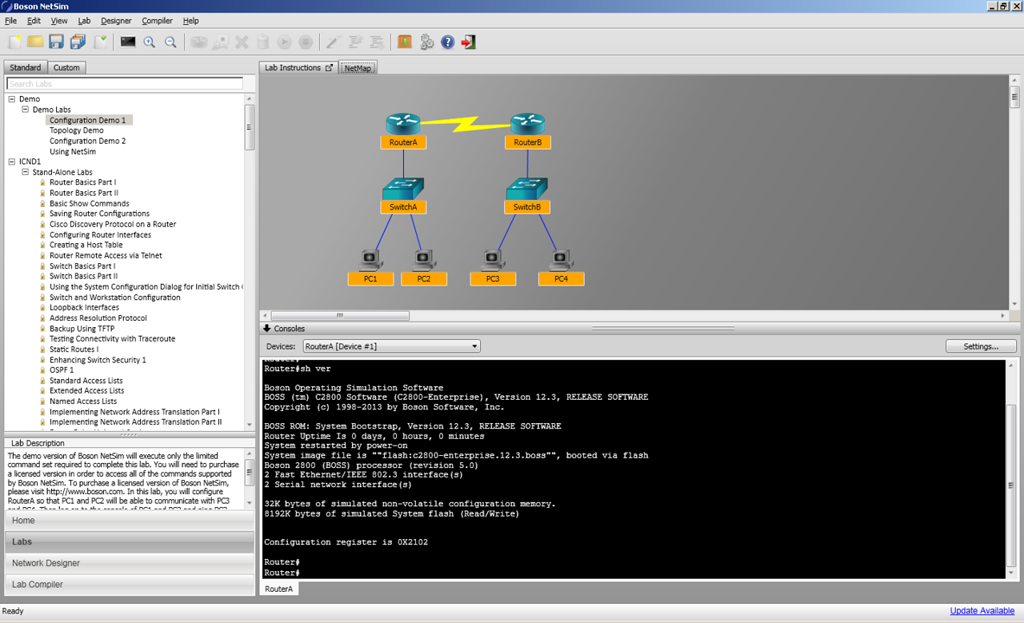
\includegraphics[width=0.9\linewidth]{pic/netsim}
	\caption{Boson NetSim}
	\label{fig:netsim}
	\end{figure}
		
	Основные возможности Boson NetSim:
	
	\begin{itemize}
		\item Поддерживает 42 маршрутизатора, 6 коммутаторов и 3 других устройства
		\item Симулирует сетевой трафик с помощью технологии виртуальных пакетов
		\item Предоставляет два различных стиля просмотра: режим Telnet'а или режим подключения по консоли
		\item Поддерживает до 200 устройств на одной топологии
		\item Позволяет создавать свои собственные лаборатории
		\item Включает в себя лаборатории, которые поддерживают симуляцию SDM
		\item Включает в себя не-Cisco устройства, такие как TFTP Server, TACACS + и генератор пакетов (это, вероятно, те самые 3 других устройства)
	\end{itemize}
	
	
	Недостатки у него те же, что и в Packet Tracer.
	
	Итог?
	— Тем, кому не жалко определенной суммы, и при этом не хочется разбираться и создавать свои топологии, а хочется просто попрактиковаться перед экзаменом, будет очень кстати.
	
	\section{Cisco IOU}
	
	Ну и наконец знаменитый Cisco IOU (Cisco IOS on UNIX) — это проприетарный софт, который официально не распространяется вообще никак.
	
\begin{figure}[h!]
\centering
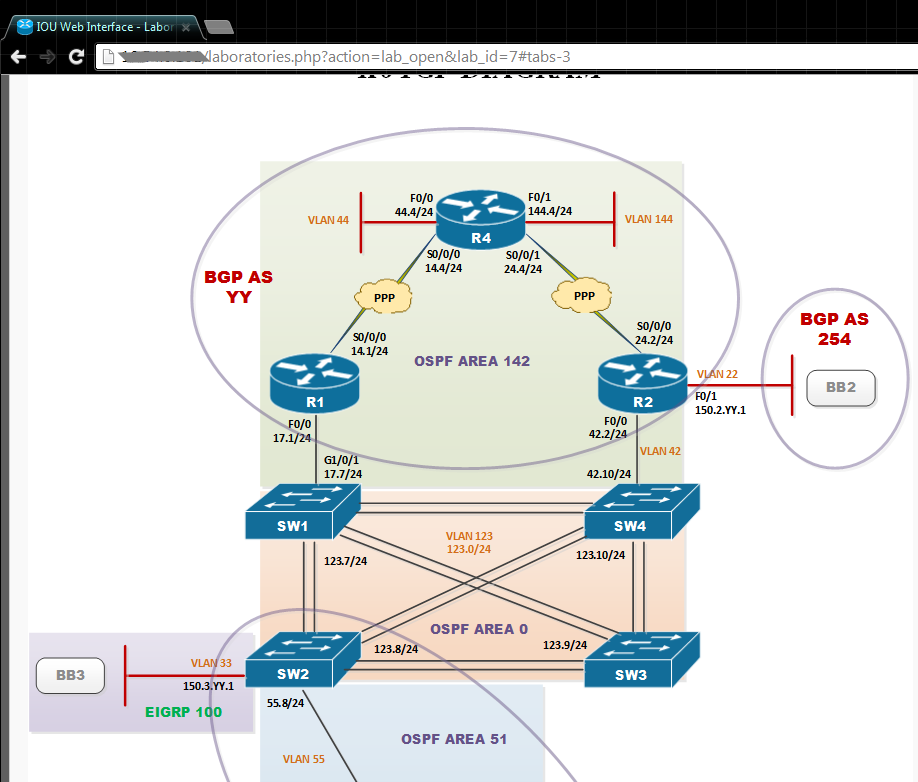
\includegraphics[width=0.7\linewidth]{pic/ciscoIOU}
\caption{Cisco IOU}
\label{fig:ciscoIOU}
\end{figure}
	
	Существует мнение, что Cisco может отследить и идентифицировать того, кто использует IOU.
	При запуске происходит попытка HTTP POST запроса на сервер xml.cisco.com.
	Данные, которые при этом отправляются, включают в себя hostname, логин, версию IOU и т.д.
	
	Известно, что Cisco TAC использует именно IOU.
	Эмулятор пользуется большой популярностью у тех, кто готовится к сдаче CCIE.
	Изначально работал только под Solaris, но со временем был портирован и на Linux.
	Состоит из двух частей — l2iou и l3iou, по названию можно догадаться, что первый эмулирует канальный уровень и коммутаторы, а второй — сетевой и маршрутизаторы.
	
	Конфигурирование проводится путем редактирования текстовых конфигурационных файлов, но некоторое время назад для него был разработан и графический интерфейс, веб фронтенд.	
	
	Интерфейс достаточно интуитивен, с его помощью можно производить практически все действия.
	
	Запуск вот такой топологии (см. рис. \ref{fig:topologyCCIE}) приводит всего лишь к 20\% загрузке CPU.	
	
	\begin{figure}[h!]
	\centering
	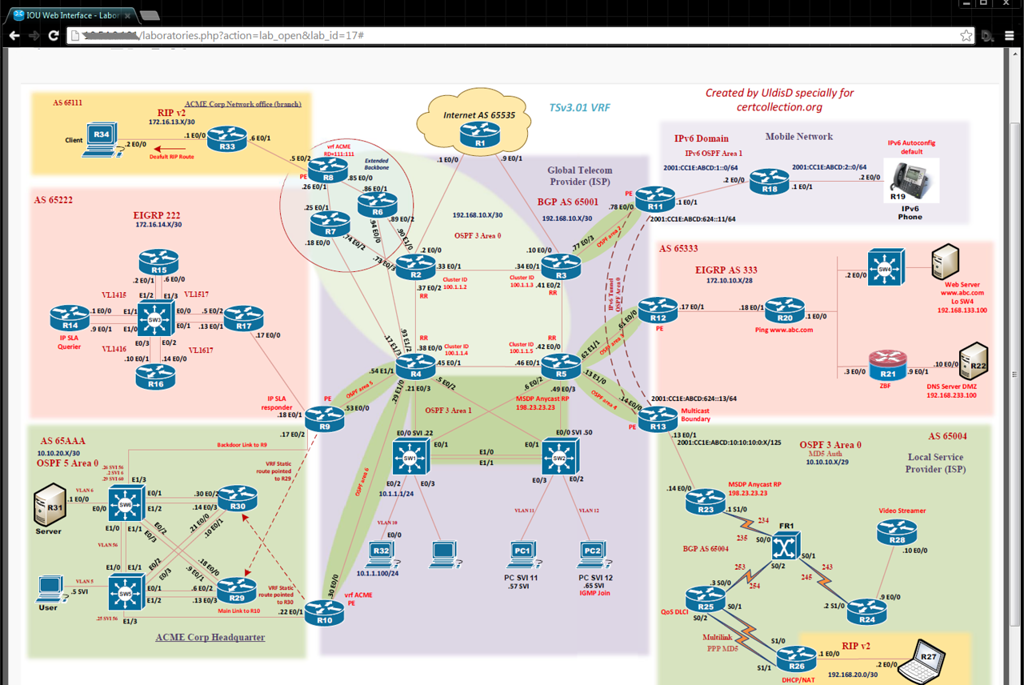
\includegraphics[width=0.7\linewidth]{pic/topologyCCIE}
	\caption{}
	\label{fig:topologyCCIE}
	\end{figure}
		
	К слову, это топология для подготовки к сдаче CCIE.
	
	Для того чтобы подключиться к любому устройству на схеме, достаточно просто кликнуть на нем и сразу же откроется putty.
	
	
	
	Возможности IOU действительно очень большие.
	Хотя и не без недостатков, некоторые проблемы на канальном уровне все же имеются.
	В некоторых, к примеру, невозможно жестко выставить дуплекс, но это всё мелочи — весь основной функционал работает, и работает отлично.
	
	\chapter*{Заключение}
	\addcontentsline{toc}{chapter}{ЗАКЛЮЧЕНИЕ}
	
	Актуальность темы дипломной работы определяется быстрым ростом количества компаний, имеющих сложную информационную структуру. Наряду с этим возникает необходимость настройки огромного количества активного сетевого оборудования.	
	Все эти факторы приводят к тому, что администраторам информационной инфраструктуры компании приходится тратить много времени на порой рутинные работы.
	
	Цель дипломной работы состоит в разработке системы для автоматизированного создания конфигурационных файлов оборудования.
	
	Поставленная цель обусловила следующие задачи дипломной работы:
	
	\begin{itemize}
		\item определить сущности проектируемой системы и архитектуру их взаимодействия;
		\item реализовать систему в виде кроссплатформенного приложения с графическим интерфейсом;
		\item провести тестированием в лабораторной среде.
	\end{itemize}
	
	Объектом исследования выступает сетевое оборудование Cisco Systems.
	
	Предметом исследования в дипломной работе являются современные средства коммуникации и их интеграция в методы управления информационной инфраструктурой для повышения таких аспектов информационной безопасности предприятия, как целостность и доступность.
	
	Теоретическая значимость дипломного исследования состоит в развитии и совершенствовании методологии управления оборудованием информационной инфраструктуры предприятия.
	
	Практическая значимость работы определяется тем, что ее результаты позволяют повысить степень эффективности управления информационной инфраструктурой предприятия и снизить связанные с этим операционные расходы при использовании разработанной системы, направленной на повышение уровня таких аспектов администрирование, как быстрота и легкость обслуживания.
	
	Новизна дипломной работы заключается в разработке и реализации кроссплатформенной модели автоматизации конфигурирования оборудования.
	
	
	\appendix
	
	
	\titleformat{\chapter}[hang]
	{\filleft}
	{}{1pt}{\MakeUppercase}
%	
%
%	
%	\newappendix{Пример приложения}


	\renewcommand{\bibname}{Список использованной литературы}
	\addcontentsline{toc}{chapter}{\bibname}
	\bibliographystyle{plain}
	\bibliography{bib/lit}	
\end{document}    